\chapter{Composing a solver}
\label{chapter:composingats}
\smtrat contributes a toolbox for composing an SMT compliant solver for real arithmetic, that means it 
is incremental, supports backtracking and provides reasons for inconsistency. The resulting
solver is either a fully operative SMT solver for real arithmetic, which can be applied
directly on \texttt{.smt2}-files, or a theory solver, which can be embedded into an SMT 
solver in order to extend its supported logics by real arithmetic.

We are talking about composition and toolbox, as \smtrat contains implementations
of many different mathematical approaches to tackle real arithmetic, each of them
embedded in a module with uniform interfaces. Theses modules form the tools in the toolbox
and it is dedicated to a user how we use them for solving a real arithmetic formula.
We provide a self-explanatory graphical user interface (GUI) for defining a graph-based 
strategy specifying which module(s) should be applied on which formula, 
taking into account the modules we have already involved.

In Section~\ref{sec:managerstrategy} we have already introduced
a strategy and in the following of this chapter we firstly give a brief introduction 
to the existing modules equipped with an estimation of their input-based performances and then illustrate
how to use the GUI for composing a strategy.

\section{Existing module implementation}
\subsection{The \texttt{CNFerModule}}
\subsection{The \texttt{PreprocessingModule}}
\subsection{The \texttt{SATModule}}
\subsection{The \texttt{LRAModule}}
\subsection{The \texttt{GBModule}}
\subsection{The \texttt{VSModule}}
\subsection{The \texttt{CADModule}}

\section{Specifying a strategy with the GUI}

The presented GUI is called SMT-XRAT. The GUI possesses an own name to highlight, that it is a standalone program apart of the actual toolbox. The name simply derives from SMT-RAT and adds the letter `X' to symbolize, that it is a graphical window application, whereas the toolbox is operated in the console.

The following subsections are used to give an overview of SMT-XRAT and to introduce its functionalities. Besides the required features, additional features are stated, which have been implemented to gain a higher degree of usability and user experience. These features help to prevent user frustrations, enable fail-safe working and support the visual creation and manipulation process of strategy graphs.

\subsection{Concept}
\label{sec:concept_of_smt-xrat}
The underlying concept of SMT-XRAT is the user-guided, visual modeling of module compositions in form of graphs and their mapping onto their corresponding source code for SMT-RAT. A modeled graph expresses an intended strategy graph of the user. Both can easily be projected on each other, because the data structure of a strategy graph also describes a graph structure, as explained in the previous chapter. A mapping considers not only the modeled hierarchy of the SMT-RAT modules, but also their attributes. Furthermore the GUI complies the constraints of these attributes during the modeling process, for example priority values are required to be unique.

The user benefits from that concept, because strategy graphs can be created and manipulated completely independent of SMT-RAT. No knowledge of the inner data structure of strategy graphs and no knowledge about their corresponding source code is required by the user. The GUI does not only support the visual creation of strategy graphs and their translation into source code, but also enables the user to integrate the translated source code into SMT-RAT or, if necessary, delete it subsequently. The conclusive work only involves a recompilation of SMT-RAT with the desired strategy graph instance to obtain a customized SMT solver.

SMT-XRAT has been implemented with the programming language Java. It embeds the freely available Java Universal Network/Graph Framework (JUNG) \cite{JUNG}, which fulfills the main demands of the underlying concept, as it allows to model and visualize data, which can be represented as a graph. The JUNG library helped to reduce the basic workload of the GUI creation enormously. Even though, a lot of effort still remained in adjusting its classes to fit for SMT-XRAT.

\subsection{Main window structure}
\label{sec:main_window_structure_of_smt-xrat}
The main window structure of the SMT-XRAT application can be seen in Figure \ref{fig:smt-xrat_main_window}. It principally consists only of one large pane, which is called \emph{strategy graph pane}. This pane embodies the workspace of the user and visualizes the composition of SMT-RAT modules, which are currently modeled. Only a comparatively small area is occupied by a compact menu bar, which offers further necessary or practical functionalities, but which need no visualizations, for instance the exportation of a strategy graph into SMT-RAT.
\begin{figure}
  \begin{center}
    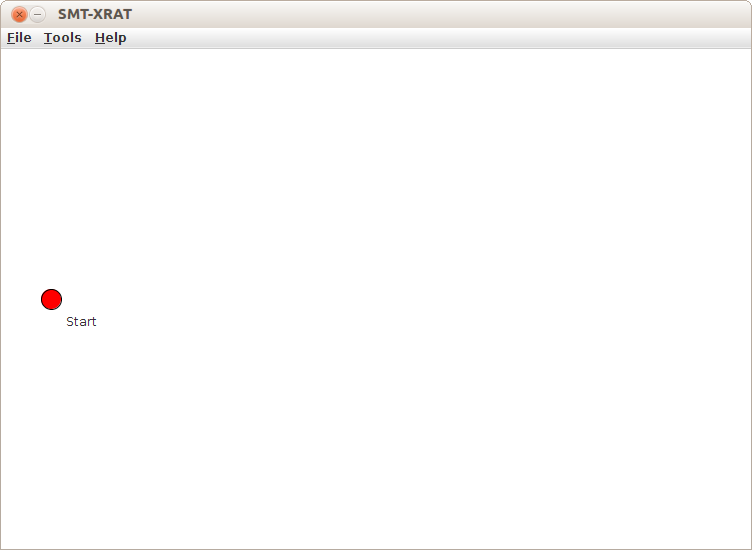
\includegraphics[width=0.9\textwidth]{graphics/smt-xrat_main_window.png}
  \end{center}
  \caption{The main window of the SMT-XRAT application in its initial state.}
  \label{fig:smt-xrat_main_window}
\end{figure}

\subsection{Strategy graph pane}
\label{sec:the_strategy_graph_pane}
The strategy graph pane is the focus point of the main window and occupies nearly all of its area. It can hereby offer enough workspace to the user to model strategy graphs without distractions. Modeled graphs are acyclic, directed and weakly connected, right as they are needed for Grammar ${\cal SG}$. Nodes represent SMT-RAT modules and edges represent the call hierarchy of them. Both of the element types are labeled to display all necessary and editable module attributes within the visualization. Thereby the user is always able to keep a full overview of the modeled strategy graph and its attributes. Moreover, the user can continuously be aware of the presented execution flow of the module composition. Thus, SMT-XRAT nicely supports the user to visualize an imagined strategy while mapping it onto a data structure in the same time.

Modeling strategy graphs on the pane implies the interactive operations of adding, editing and deleting modules and also aligning elements, if desired by the user.

\subsubsection{Adding backends}
\label{sec:adding_backends}
\begin{figure}
  \begin{center}
    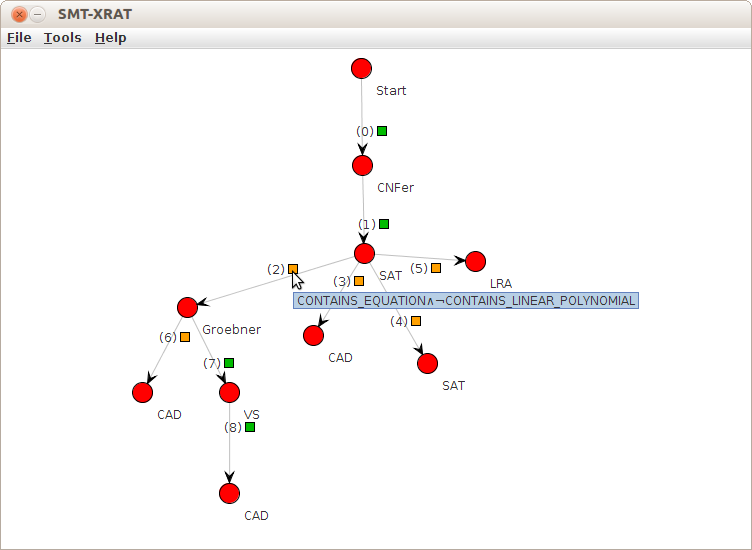
\includegraphics[width=0.9\textwidth]{graphics/smt-xrat_condition_ttt.png}
  \end{center}
  \caption{The small rectangles alongside the edges reveal the hidden condition of a backend.}
  \label{fig:smt-xrat_condition_ttt}
\end{figure}

An initial visualization of the pane contains the inevitable \emph{Start} module of an SMT solver, which displays no attributes, but marks the starting point for the user to create the desired strategy graph. The user can simply consider the \emph{Start} module as the frontend of an SMT solver where NRA problems are passed to. Building up a composition of modules occurs by appending backends to the \emph{Start} module and then to the newly appended backends and so forth. When appending a backend to a selected module, a dialog window requests the operating user to input a condition and to choose the type of SMT-RAT module for the new backend. The GUI provides a special input interface to enter conditions, which is explained later. For each appended backend a new node as well as a directed edge from the originating module to this new node is drawn in the visualization. In this way, the graph gradually arises on the pane. The added graph elements display the inputted data of a backend. A node is labeled with 
its 
type of SMT-RAT module whereas an edge holds its condition and an automatically assigned priority value. Initially this priority value is always the total number of currently existing modules decreased by 1, as the \emph{Start} module is not counted. As inputted conditions might get quite long, they cannot be directly seen on the strategy graph pane. Instead, a small rectangle alongside the edge reveals them quickly on request. The user needs to point the mouse cursor over a rectangle to obtain its corresponding tool tip text, which shows the hidden condition, as can be seen in Figure \ref{fig:smt-xrat_condition_ttt}. This leaves the graph compact and helps to concentrate on the more essential aspect of modeling an execution hierarchy. The user can choose to input an own condition or leave it by the default value of `\texttt{TRUE}', which, as described in the last 
chapter, means that a condition is always satisfied. To point out better which modules contain default conditions and which do not, the color of a rectangle containing a default condition is green and otherwise orange. When looking at the strategy graph pane, the user is always capable to recognize the execution flow of the modules by following the directed edges in the graph. The colored rectangles signalize at which points of the hierarchy a passed formula must be checked against the condition for an intended backend. This is a quite handy feature, when the user wants to re-enact the solving of an SMT problem.

\subsubsection{Grammar for conditions}
\label{sec:grammar_for_backend_conditions}
When adding a module to the strategy graph pane, the user has to input a valid condition for its intended use as backend. A valid condition is a derivation of the formal Grammar $\cal C$, which completes Grammar $\cal SG$ of Definition \ref{def:grammar_strategy_graph} of the previous chapter. The grammar is concretely utilized by the GUI. A recursive descent parser \cite{ALSU07} has been implemented in the GUI, which applies exactly this grammar.
Conditions are derived from the formal Grammar $${\cal C}=(N, \Sigma, R, S).$$ The set of nonterminals is given by $$N=\{S, T, B, C, D, P\},$$ whereas the set of terminal symbols $$\Sigma=\{\texttt{(}, \texttt{)}, \neg, \leftrightarrow, \oplus, \rightarrow, \land, \lor\} \cup \{\texttt{TRUE}, \texttt{p}_1, \dots, \texttt{p}_n \}$$ consists of the union of logical operators and propositions. $S \in N$ is the start symbol of the production rules denoted by the set $R$, which covers the following:
\begin{center}
\begin{tabular}{lccccccccccc}
  $S$ & $\rightarrow$ & \texttt{TRUE} & $|$ & $T$ & $|$ & $C$ & $|$ & $D$ & $|$ & $TBT$ \\
  $T$ & $\rightarrow$ & $P$ & $|$ & $\neg T$ & $|$ & \texttt{(}$C$\texttt{)} & $|$ & \texttt{(}$D$\texttt{)} & $|$ & \texttt{(}$TBT$\texttt{)} \\
  $B$ & $\rightarrow$ & $\leftrightarrow$ & $|$ & $\oplus$ & $|$ & $\rightarrow$ \\
  $C$ & $\rightarrow$ & $C\land C$ & $|$ & $T$ \\
  $D$ & $\rightarrow$ & $D\lor D$ & $|$ & $T$ \\
  $P$ & $\rightarrow$ & $\texttt{p}_1$ & $|$ & \dots & $|$ & $\texttt{p}_n$ \\
\end{tabular}
\end{center}

The nonterminal symbols stay for the following: As said, $S$ for the start symbol of the production rules, $T$ for term, $B$ for binary operator, $C$ for conjunction, $D$ for disjunction and $P$ for proposition.

The terminals `$\neg$', `$\leftrightarrow$', `$\oplus$', `$\rightarrow$', `$\land$' and `$\lor$' represent their related logical operators, which, in the context of conditions, are negation, equivalence, exclusive or, implication, conjunction and disjunction respectively. Their semantics is defined as usual. The terminal symbols `\texttt{(}' and `\texttt{)}' are used, in case several different types of logical operators are utilized within one term. They point out the precedences of the operators in the same way as it is known from mathematical contexts. For example, for the term $p_1 \lor p_2 \land p_3$ it is unknown, which of the logical operators has the higher precedence. Writing the same term with parenthesis as $p_1 \lor (p_2 \land p_3 \texttt{)}$ clarifies, that the conjunction operator is of higher precedence.

The propositions $P = \{p_1, \dots, p_n\}$ are not concretely mentioned in the grammar, as they have already exemplary been listed in Chapter \ref{chap:the_smt-rat_application} and numerous are available. Furthermore, the set of available propositions can vary among releases of the toolbox, as well as the user can also define own propositions. For this reason, the set of propositions is dynamically loaded from the SMT-RAT source code each time the GUI is started. As mentioned in the previous chapter, the set of SMT-RAT modules can vary as well. Therefore the list of available SMT-RAT modules is also dynamically loaded. This allows to edit SMT-RAT without editing the GUI additionally.

The grammar is constructed in such a manner, that the user working in the context of SMT solving is naturally enabled to input conditions effortlessly, although they must be derivable from the grammar. Therefore it can be assumed that no additional workload arises.

\subsubsection{Improved interface for inputting conditions}
\label{sec:improved_interface_for_inputting_conditions}
When adding backends to existing modules on the strategy graph pane, a dialog window requests the user to input a desired condition, which must be derivable from the above defined Grammar $\cal C$. This dialog window is equipped with additional features to ease the input process for the user and to improve the usability. A specialized text area is used for inputting conditions. Initially, it contains the default proposition value `\texttt{TRUE}'. The window also contains a combo box, where the user has the possibility to choose a proposition value from. A chosen proposition value can then be copied to the current caret position of the text area. Should the occasion arise that the user selects a part of an entered condition beforehand, it is simply overwritten by the chosen proposition value. The user can only input proposition values by using this combo box. Proposition values cannot be typed into the text area directly. On the one side, this simply prevents mistyping and, on the other side, the list of 
propositions might be changed between releases of SMT-RAT, as stated above. The combo box informs the user about all currently available propositions of the toolbox. In many cases it will not be sufficient to use conditions, which contain just one single proposition. When requiring a Boolean combination of conditions, the above stated logical operators are needed. Although, the characters of the operators are generally not present on a keyboard, they can just be typed into the specialized text area of the dialog window. To input the conjunction operator `$\land$', for instance, the user simply needs to hit the key `c' on the keyboard. Instead of the character `c', the character `$\land$' will then appear in the text area. The mapping between the symbols, which express the given logical operators, and characters, which are present on general keyboards, supports the readability and comprehension of inputted terms and therefore achieves a better user experience.

In order to increase the user experience even further, the text area treats the single characters of an inputted proposition value as a block, which cannot be entered by the caret of the text area. This means, that if the caret is positioned directly left of an inputted proposition value and the user navigates the caret to the right, it will jump to the position directly right of the proposition. The caret will never appear between the characters of a single proposition value. This is the analogous case for selecting and deleting proposition values. All characters of a proposition value are always selected, deselected or deleted at once. This allows a faster and more comfortable navigation and editing.

The text area allows to copy and paste conditions or parts of it. Text, which should be pasted into the text area, is checked to guarantee, that it only contains allowed values. Otherwise it will be refused. Allowed values cover proposition values, the characters used to express logical operators and parenthesis.

When the user confirms the dialog window, the implemented recursive descent parser of SMT-XRAT checks, whether the inputted condition is a valid derivation of Grammar $\cal C$ or not. In case it is not, the user will be returned to the dialog window to re-edit the condition, as can be seen in Figure \ref{fig:smt-xrat_condition_wrong}. Otherwise the inputted condition is adopted for the backend. This fail-safe method of inputting conditions saves frustrations on the side of the user. A mistake is better pointed out at this stage than at the time of exporting the strategy graph or even when compiling the resulting SMT solver. The user is promptly informed about an error and is directly enabled to correct it.
\begin{figure}
  \begin{center}
    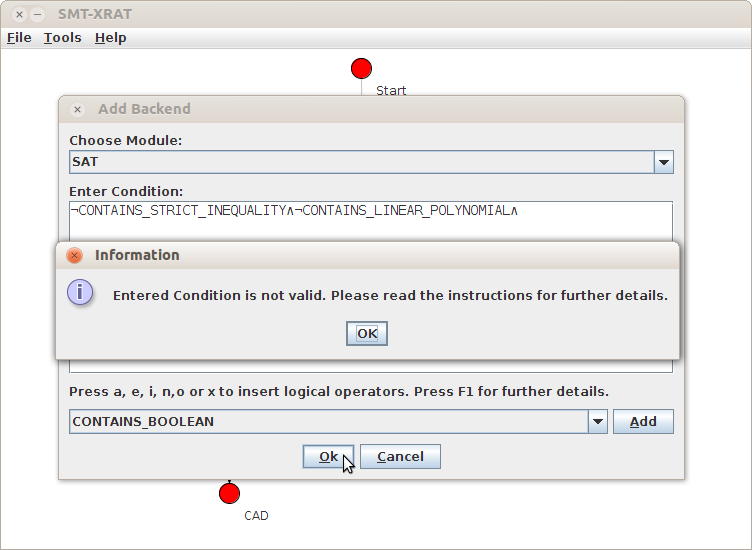
\includegraphics[width=0.9\textwidth]{graphics/smt-xrat_condition_wrong.png}
  \end{center}
  \caption{A wrong condition has been inputted by the user.}
  \label{fig:smt-xrat_condition_wrong}
\end{figure}

\subsubsection{Manipulating the strategy graph}
\label{sec:manipulating_the_strategy_graph}
Besides the capability of adding modules, the strategy graph pane gives the user also the possibility to remove and edit them subsequently.

The deletion of a single module implicates that all of its succeeding modules in the composition hierarchy will be removed as well. The strategy graph pane is only allowed to contain one single weakly connected graph. Furthermore, when deleting one or implicitly more modules, the priority values of all remaining modules might automatically be adjusted to comply the constraints of the priority values. However, the logical priority order remains untouched.

When editing modules, the same dialog window is displayed as for adding modules. The window components are already filled in with the attributes of the corresponding module. However, priority values are not manipulated via this dialog window. As said before, priority values are automatically assigned, when a module is created, and they are displayed alongside the edges. The user can manually change the priority order by pushing the priority value of a lower prioritized module in front of the priority value of a higher prioritized one. The user achieves this by using the mouse pointer to draw a dashed arrow from the edge label of that lower prioritized module to the edge label of the higher prioritized module, as it is illustrated by Figure \ref{fig:smt-xrat_priority_a}. Afterwards the lower prioritized module will have a higher priority than the other one. The priority values of the modules might just be swapped. If this is not possible, the priority values of the modules and of their 
preceding modules are adjusted automatically, so that as a result, the newly prioritized module will be ordered logically before the other one. The adaptation of the priority values is emphasized by Figure \ref{fig:smt-xrat_priority_b}. This mechanism has been implemented not only to offer a fast way of subsequently changing priority values, but also to picture the actions of the user even more.
\begin{figure}
  \begin{center}
    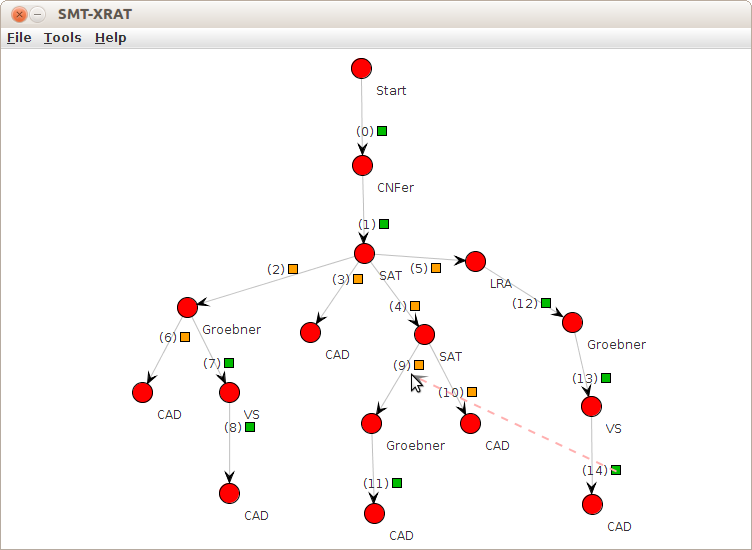
\includegraphics[width=0.9\textwidth]{graphics/smt-xrat_priority_a.png}
  \end{center}
  \caption{Priority values before changes are set.}
  \label{fig:smt-xrat_priority_a}
\end{figure}

\begin{figure}
  \begin{center}
    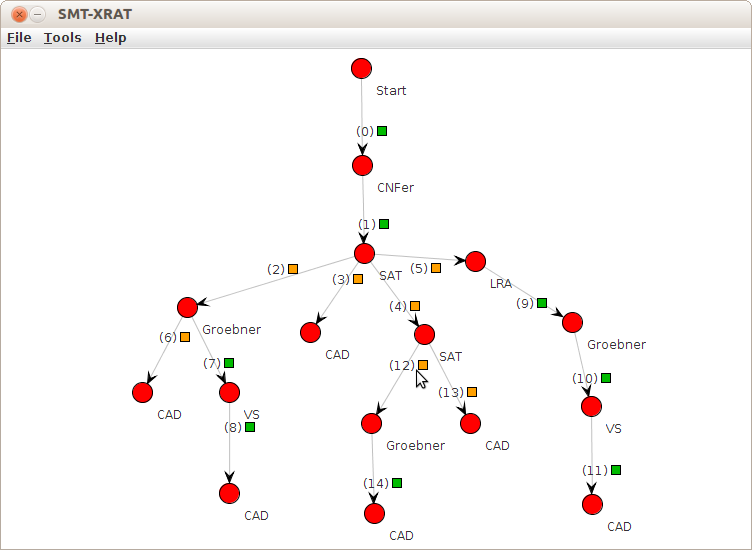
\includegraphics[width=0.9\textwidth]{graphics/smt-xrat_priority_b.png}
  \end{center}
  \caption{Intentionally changed and automatically adapted priority values.}
  \label{fig:smt-xrat_priority_b}
\end{figure}

Note that graph elements or even a group of graph elements can be positioned freely on the strategy graph pane anytime after there creation.

\subsection{Further functionalities}
\label{sec:further_functionalities}
Further features of the GUI are reached through the menu bar. The most important and also necessary functionality is the management of strategy graphs inside the SMT-RAT source code. It is not sufficient to design a strategy graph on the pane. Its underlying data structure also needs to be translated into source code, which must then be integrated into SMT-RAT. To export a currently modeled strategy graph, the user simply needs to open the corresponding dialog window and choose a name, Figure \ref{fig:managing_smt_solvers} shows an example for exporting the current strategy graph and naming it \emph{SMT\_XRAT}. The GUI will then fulfill the translation and integration process. The same dialog window also lists all existing strategy graphs, which are currently integrated in the source code, and gives the opportunity to delete them separately. This can be seen for the existing strategy graph \emph{NRATSolver} of the example.

The remaining features hold by the menu bar are not mandatory, but improve the creation process and usability. For example, the GUI allows the user to save the current strategy graph into an XML file. This file can then be opened again for later editing or it can be exchanged with another user. Another practical feature is the ability to save a screen shot of the strategy graph pane into an image file. Such image files can be used to discuss strategy graphs, when it is not desired to run the GUI. For this purpose, it could be attached into an email or included into a presentation, for instance.
\begin{figure}
  \begin{center}
    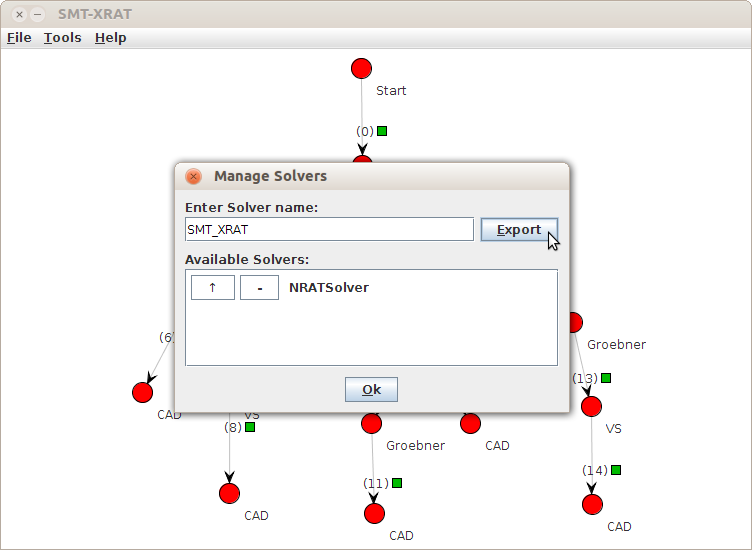
\includegraphics[width=0.9\textwidth]{graphics/smt-xrat_manage_solvers.png}
  \end{center}
  \caption{Managing SMT solvers in the SMT-RAT source code.}
  \label{fig:managing_smt_solvers}
\end{figure}


